% !TEX TS-program = pdflatex
% !TEX encoding = UTF-8 Unicode

% This is a simple template for a LaTeX document using the "article" class.
% See "book", "report", "letter" for other types of document.

\documentclass[11pt]{article} % use larger type; default would be 10pt

\usepackage[utf8]{inputenc} % set input encoding (not needed with XeLaTeX)

%%% Examples of Article customizations
% These packages are optional, depending whether you want the features they provide.
% See the LaTeX Companion or other references for full information.

%%% PAGE DIMENSIONS
\usepackage{geometry} % to change the page dimensions
\geometry{a4paper} % or letterpaper (US) or a5paper or....
% \geometry{margin=2in} % for example, change the margins to 2 inches all round
% \geometry{landscape} % set up the page for landscape
%   read geometry.pdf for detailed page layout information

\usepackage{graphicx} % support the \includegraphics command and options

% \usepackage[parfill]{parskip} % Activate to begin paragraphs with an empty line rather than an indent

%%% PACKAGES
\usepackage{booktabs} % for much better looking tables
\usepackage{array} % for better arrays (eg matrices) in maths
\usepackage{paralist} % very flexible & customisable lists (eg. enumerate/itemize, etc.)
\usepackage{verbatim} % adds environment for commenting out blocks of text & for better verbatim
\usepackage{subfig} % make it possible to include more than one captioned figure/table in a single float
% These packages are all incorporated in the memoir class to one degree or another...

%%% HEADERS & FOOTERS
\usepackage{fancyhdr} % This should be set AFTER setting up the page geometry
\pagestyle{fancy} % options: empty , plain , fancy
\renewcommand{\headrulewidth}{0pt} % customise the layout...
\lhead{}\chead{}\rhead{}
\lfoot{}\cfoot{\thepage}\rfoot{}

%%% SECTION TITLE APPEARANCE
\usepackage{sectsty}
\usepackage{tabularx}
\allsectionsfont{\sffamily\mdseries\upshape} % (See the fntguide.pdf for font help)
% (This matches ConTeXt defaults)

%%% ToC (table of contents) APPEARANCE
\usepackage[nottoc,notlof,notlot]{tocbibind} % Put the bibliography in the ToC
\usepackage[titles,subfigure]{tocloft} % Alter the style of the Table of Contents
\renewcommand{\cftsecfont}{\rmfamily\mdseries\upshape}
\renewcommand{\cftsecpagefont}{\rmfamily\mdseries\upshape} % No bold!

%%% END Article customizations

%%% The "real" document content comes below...

\title{Internship project group behavior proposal}
\author{Cees-Jan Nolen, Robert Kraaijeveld, Steven Schenk}
\date{28-9-16}

\begin{document}
  \pagenumbering{gobble}
  \maketitle
  \newpage
  \pagenumbering{arabic}
  \tableofcontents

\newpage
\section{Introduction}
In this document, we will be presenting our concept for the implementation of group behavior within our internship project. Since group behavior and the deeper themes of friendship and group forming in humans are subjects that we have no experience in, we wanted to present our concept to you first to see whether our assumptions match reality. 

\section{Friendship system}
In order to make our room filled with NPC's seem more like a room filled with humans, we intend to implement a friendship system. 

~\\
In real life, people with common interests, backgrounds and personalities tend to become friends. Since we have only personality (for now) to distinguish our NPC's, we will let NPC's select friends based on the 'Repulsion Theory' [1] which in its' most basic form states that we are usually repulsed of people when they have dissimilar attitudes to ours.

~\\
Within our system, we represent this by using the (accumulated) personality values of NPC's who could potentially become friends. We realize that the term 'friend' is not really appropriate here, since deep friendship can arguably be said to consist of more than just common personalities. Therefore, we will be using the term 'friends' to refer to NPC's who's (accumulated) personality values are in proportion, with some margin of error.

~\\
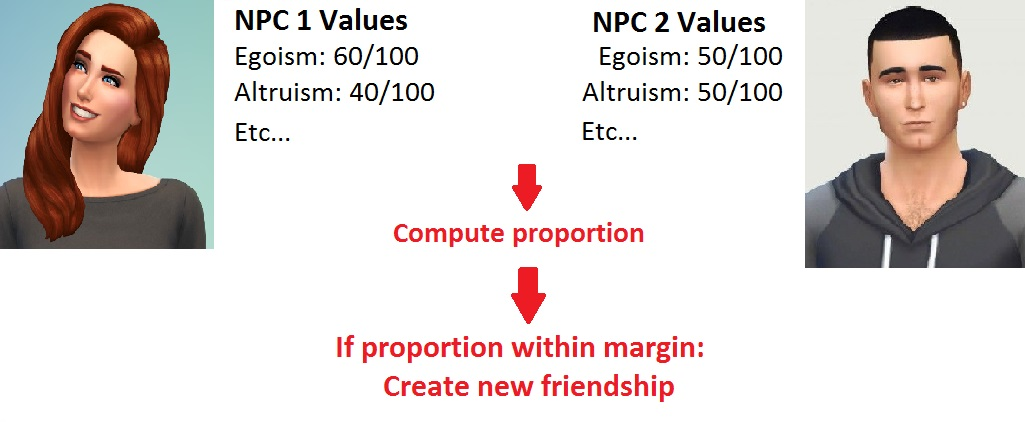
\includegraphics[scale=0.5]{friendshipCreation}

~\\
We intend for this margin of error to be changeable by the user of our project in order to allow them to customize how easily they want friendships between NPC's to form.
%WHAT DO NPC'S DO WHEN THEY ARE FRIENDS?
%EXPAND THIS

\newpage
\section{Informal groups}
As we mentioned earlier in our structure document, groups of people come in two distinct forms: Formal groups and informal groups.

~\\
Formal groups are usually found within the workplace, are created 'top-down', and are usually form edInformal groups are, as the name implies not directed or created by a formal body such as a board or a manager, but they form naturally as the human need for company arises, whether at the workplace or in a social setting. Since we do not intend to simulate a working environment in our project, we will be focusing on the latter form of groups. 

~\\
Informal groups can be loosely divided into two distinct categories: Interest groups and friendship groups.

~\\
Table 1: Differences between interest groups and friendship groups

~\\ 
\begin{tabularx}{0.7\textwidth}{ |X|X| }\hline
\textbf{Interest groups} & \textbf{Friendship groups} \\ \hline
Mutual goal & No real goal \\ \hline
Usually more hierarchic & More democratic \\ \hline
Higher purpose is more important than individual members & Group exists solely to satisfy personal member needs \\ \hline
Not necessarily common values and interests & Common ground \\ \hline
\end{tabularx}
~\\

~\\
Until we decide to implement some kind of goal seeking behavior within our NPC's (other than choosing actions that will show of their personality values) we will focus our attention on implementing a representation of friendship groups.  

\newpage
\section{An implementation of informal friendship groups}
The friendship system that we discussed earlier will be used as a bridge to introduce NPC's to groups. A group consists of NPC's who all share a friendship with at least a certain percentage of the NPC's in the group. 

~\\
For example:

~\\
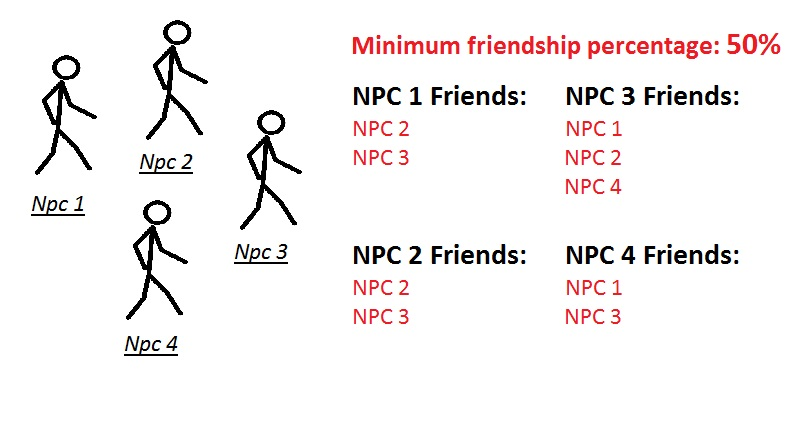
\includegraphics[scale=0.7]{group} 


~\\
A new NPC can join an existing group; Its' accumulated values are than tested against the mean\footnote{We use the mean instead of the average since this could lead to a group of egoists with one altruists having a group personality value that does not accurately represent the group members.} of all the accumulated personality values of all the group members.

~\\


\newpage
\section{References}
[1] Rosenbaum, M. E. (1986). The repulsion hypothesis: On the nondevelopment of relationships. Journal of Personality and Social Psychology, 51(6), 1156.


%NO REAL GOAL
%CONNECT GROUP BELONGING WITH BETTER EMOTIONS?
% LET GROUP PERSONALITY OVERTAKE NPC PERSONALITY?
%LET GROUP SEEK OUT ONLY BEST MATCHES BY KICING OUT AVERAGE MATCHES FOR BETTER ONES? WOULD BE A GOOD WAY TO MAKE MEMBERS LEAVE..
%USE DIFFERENT FACTORS OTHER THAN PERSONALITY FOR GROUP MEMBERSHIP DETERMINATION?
%USE SOCIAL COMPARISON/SOCIAL STATUS?

%INTEREST GROUPS: INFORMAL, BUT GOAL. WHAT KIND OF GOAL CAN WE GIVE.

%"They
% suggest that, in many social comparison situations,
% one is more likely to compare oneself with an individual
% (or group) who is "at about the same level" on given
% attributes than with an individual who is either greatly
% superior to or greatly inferior to oneself on the given
% attributes" 



\end{document}